%!TEX root = karen.tex

\chapter{Projected Weights on the Sphere} 
It is shown in \cite{FlyerWright09, FlyerLehto11} that a projection operator

$$ 
\mathbf{P} =  \mathbf{I} - \vx \vx^{T} = \begin{bmatrix} 
(1 - x^{2}) & -xy & -xz \\ 
-xy & (1 - y^{2}) & -yz \\ 
-xz & -yz & (1-z^{2})
\end{bmatrix} = \begin{bmatrix} \mathbf{p}_{x}^{T} \\ \mathbf{p}_{y}^{T} \\ \mathbf{p}_{z}^{T} \end{bmatrix}
$$
where $\mathbf{p}_{x}^{T}$ represents the projection operator in the $x$ direction. 

From \cite{FlyerWright09}, the projected RBF gradient operator is:
\begin{align}
\mathbf{P} \cdot \nabla \phi_{k}(r(\vx)) & = \mathbf{P} \cdot \frac{(\vx-\vx_{k})}{r(\vx)} \d{\phi_{k}(r(\vx))}{r(\vx)}  \nonumber \\
& = -\mathbf{P} \cdot \vx_{k}\frac{1}{r(\vx)} \d{\phi_{k}(r(\vx))}{r(\vx)}  \nonumber \\ %\label{eq:xsfc_negative}
& = \begin{bmatrix} x \vx^{T} \vx_{k} - x_{k} \\  y \vx^{T} \vx_{k} - y_{k} \\  z \vx^{T} \vx_{k} - z_{k} \end{bmatrix} \frac{1}{r(\vx)} \d{\phi(r(\vx))}{r} \label{eq:sfc_gradient_operator}.
\end{align}
The operator $\mathbf{I} - \vx \vx^{T}$ for $\vx = (x,y,z)$ projects a vector onto the plane tangent to the unit sphere at $(x,y,z)$. Therefore, Equation~\ref{eq:sfc_gradient_operator} gives the projection of the gradient operator at $\vx_{k}$ onto the plane tangent to $\vx$. 

\section{Direct Weights} 

Following \cite{FlyerLehto11}, \ref{eq:sfc_gradient_operator} takes on the following when adapted to RBF-FD:  
\begin{equation}
[ \mathbf{p}_{x} \cdot \nabla{f(\vx)}] |_{\vx = \vx_{c}} = \sum_{k=1}^{n} c_{k} \underbrace{\left[ x_{c} \vx_{c}^{T} \vx_{k} - x_{k} \right] \frac{1}{r} \d{\phi(r(x_{c}))}{r}}_{B_{c,k}^{\mathbf{p}_{x}}}. 
\label{eq:xsfc_operator_flyer_et_al}
\end{equation}
and so forth for the $\mathbf{p}_{y} \cdot \nabla, \mathbf{p}_{z}  \cdot \nabla$ operators, where $\vx_{c}$ is the stencil center and $\vx_{k}$ are stencil nodes. To compute RBF-FD weights for the $\mathbf{p}_{x} \cdot \nabla$ operator, the RHS of Equation~\ref{eq:rbffd_weight_system} is filled with elements $B_{c,k}^{\mathbf{p}_{x}}$. We will refer to this method of obtaining the weights as the \emph{direct} method due to the ability to directly compute RBF-FD weights for the operators $\mathbf{P} \cdot \nabla $, and assemble the differentiation matrices $\D_{\mathbf{p_{x}} \cdot \nabla}, \D_{\mathbf{p_{y}} \cdot \nabla}, \D_{\mathbf{p_{z}} \cdot \nabla}$ without the need to compute   and/or store other weights.

\section{Indirect Weights} 

Alternatively, one is able to compute weights \emph{indirectly} as a weighted combination of existing RBF-FD weights for the unprojected $\nabla$ operator. Here we assume that differentiation matrices to compute the components of $\nabla$ are readily available in memory: 
$$
\D_{\nabla} = \begin{bmatrix} \D_{\d{}{x}} \\ \D_{\d{}{y}} \\ \D_{\d{}{z}} \end{bmatrix},
$$
where each matrix contains weights computed with the operators of Equation~\ref{eq:rbffd_grad_weights} applied to the RHS of Equation~\ref{eq:rbffd_weight_system}.  

The differentiation matrices for $\mathbf{P} \cdot \nabla$ can then be assembled as a weighted combination of the differentiation matrices for the unprojected operator: 
\begin{equation}
\D_{\mathbf{P} \cdot \nabla} = \begin{bmatrix} \D_{\mathbf{p_{x} \cdot \nabla}} \\  \D_{\mathbf{p_{y}\cdot \nabla}} \\  \D_{\mathbf{p_{z}\cdot \nabla}} \end{bmatrix} = \begin{bmatrix} 
diag(1-X^{2}) \D_{\d{}{x}} - diag(XY) \D_{\d{}{y}} - diag(XZ) \D_{\d{}{z}} \\
- diag(XY)\D_{\d{}{x}} + diag(1-Y^{2}) \D_{\d{}{y}} - diag(YZ) \D_{\d{}{z}} \\
- diag(XZ)\D_{\d{}{x}} - diag(YZ) \D_{\d{}{y}} + diag(1-Y^{2}) \D_{\d{}{z}} 
\end{bmatrix}
\end{equation}
 where $X = \{x_{c,i}\}_{i=1}^{N}$, $Y = \{y_{c,i}\}_{i=1}^{N}$, $Z = \{z_{c,i}\}_{i=1}^{N}$ are all x-components, y-components and z-components of the stencil centers $\{\vx_{c,i}\}_{i=1}^{N}$ respectively. 

\authnote{Cleanup:}
This concept equates to classical Finite Differences where for example, the standard 5-point finite difference formula for approximating the Laplacian can be expressed a weighted combination of differences for 

Have not found in literature any mention of the fact that RBF-FD weights can be used to compose operators like this. Generally, its easier to directly compute weights and assumed to be more accurate. But how much more accurate?  

One benefit of indirect weights is conservation of memory. For example, for complex operators, a single DM on $N=1 \text{million}$ nodes and $n=101$ requires roughly $1.6$ GB of memory. If the PDE is coupled and requires 

This also allows us to compose complex operators with weights loaded from disk

$O(N*n)$ cost to assemble the indirect operators after $O(N*n^{3})$ cost of assembling direct operators means this approach has potential to save FLOPs in the long run

But the question is, how accurate is it? In situations where memory is critical and these FLOPs need to be saved (i.e., large $N$ and complicated equations), would it be useful?

\authnote{Q: how do direct vs indirect weights compare? Is the lsfc different sparsity with same approximation potentials?}
\authnote{:end}


\begin{figure}[htbp]
	\centering
	\begin{subfigure}[b]{0.425\textwidth}
	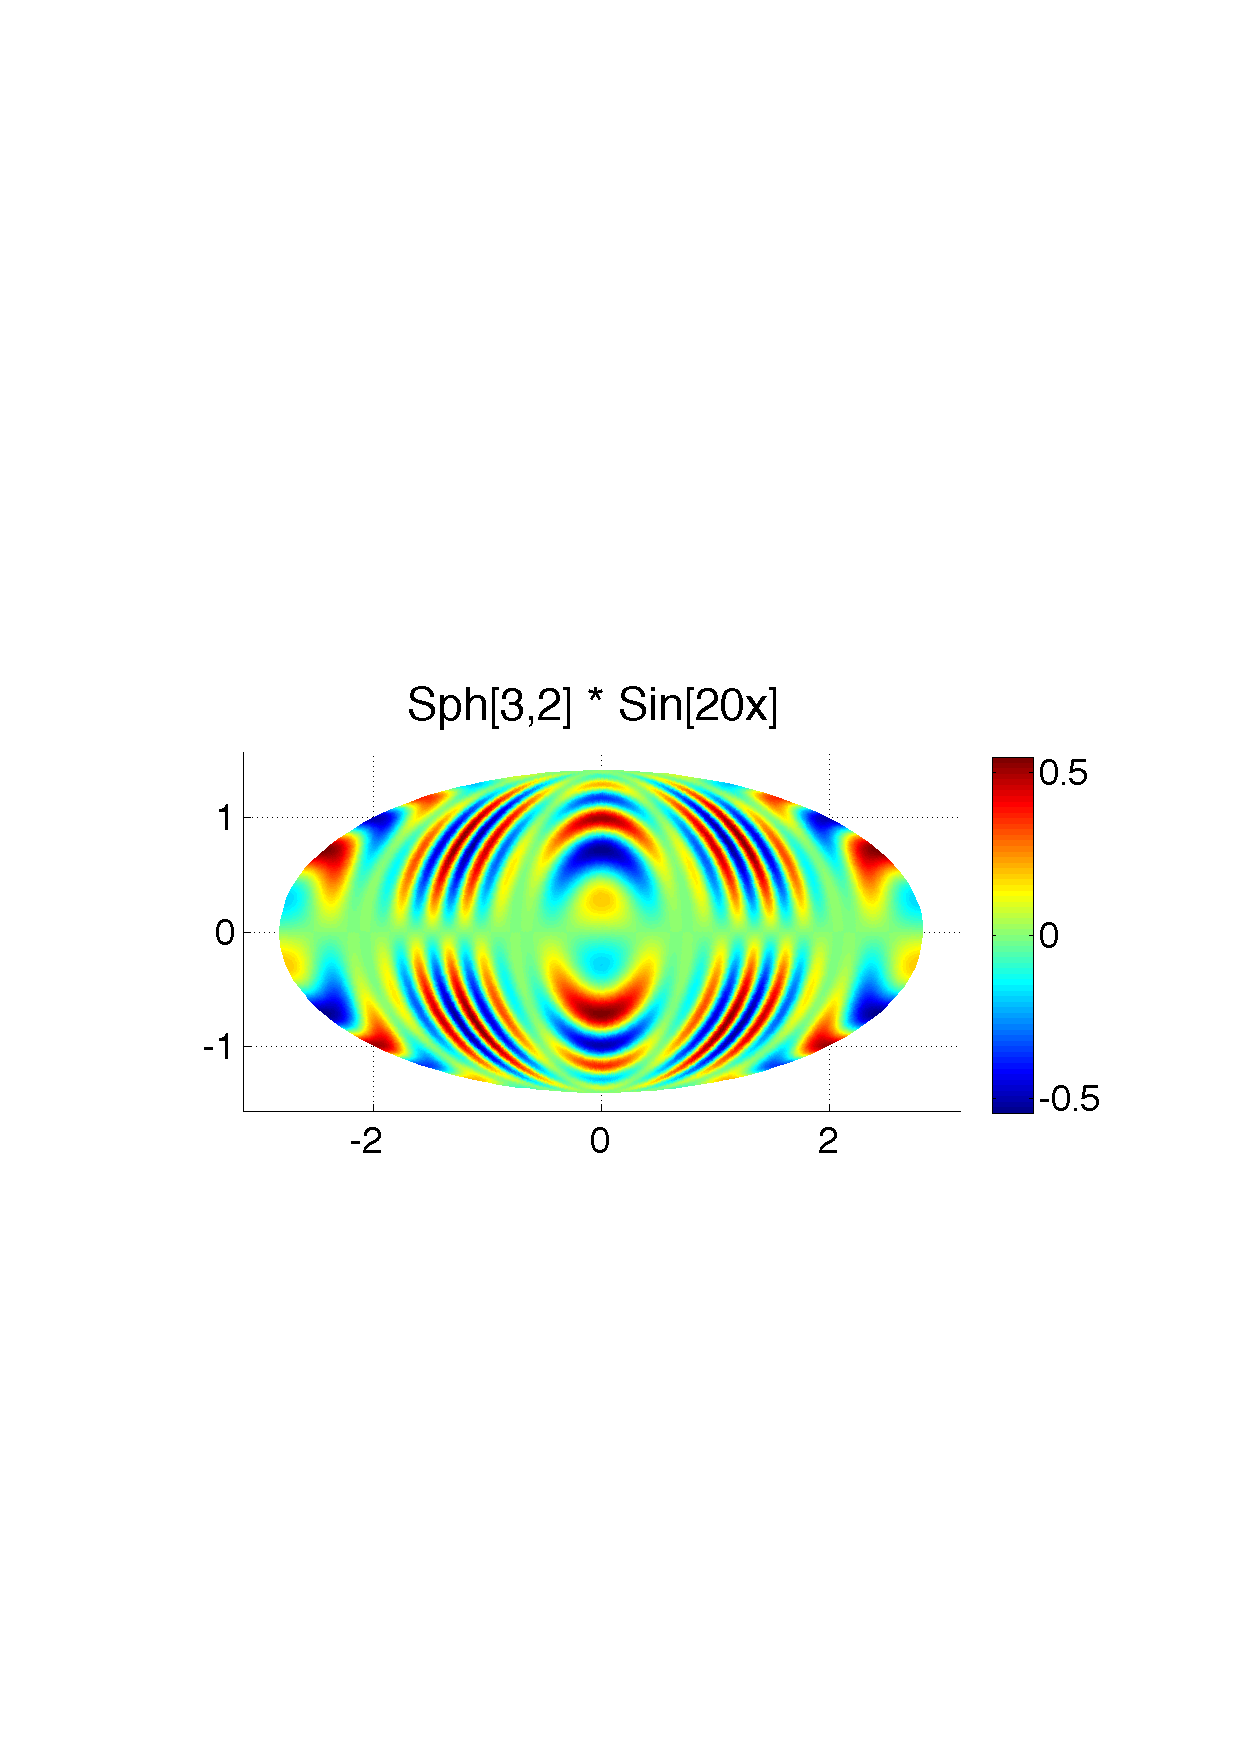
\includegraphics[width=1.0\textwidth]{../figures/chapter2/compare_weight_generation/xsfc_vs_xsfc_alt_on_sph32_times_sine_20x/sph32_times_sin20x.pdf}
	\caption{Manufactured test function: \\  $f(\vx) = Y_{3}^{2}(\vx)\sin(20x)$.  }
	\end{subfigure}
	\begin{subfigure}[b]{0.425\textwidth}
	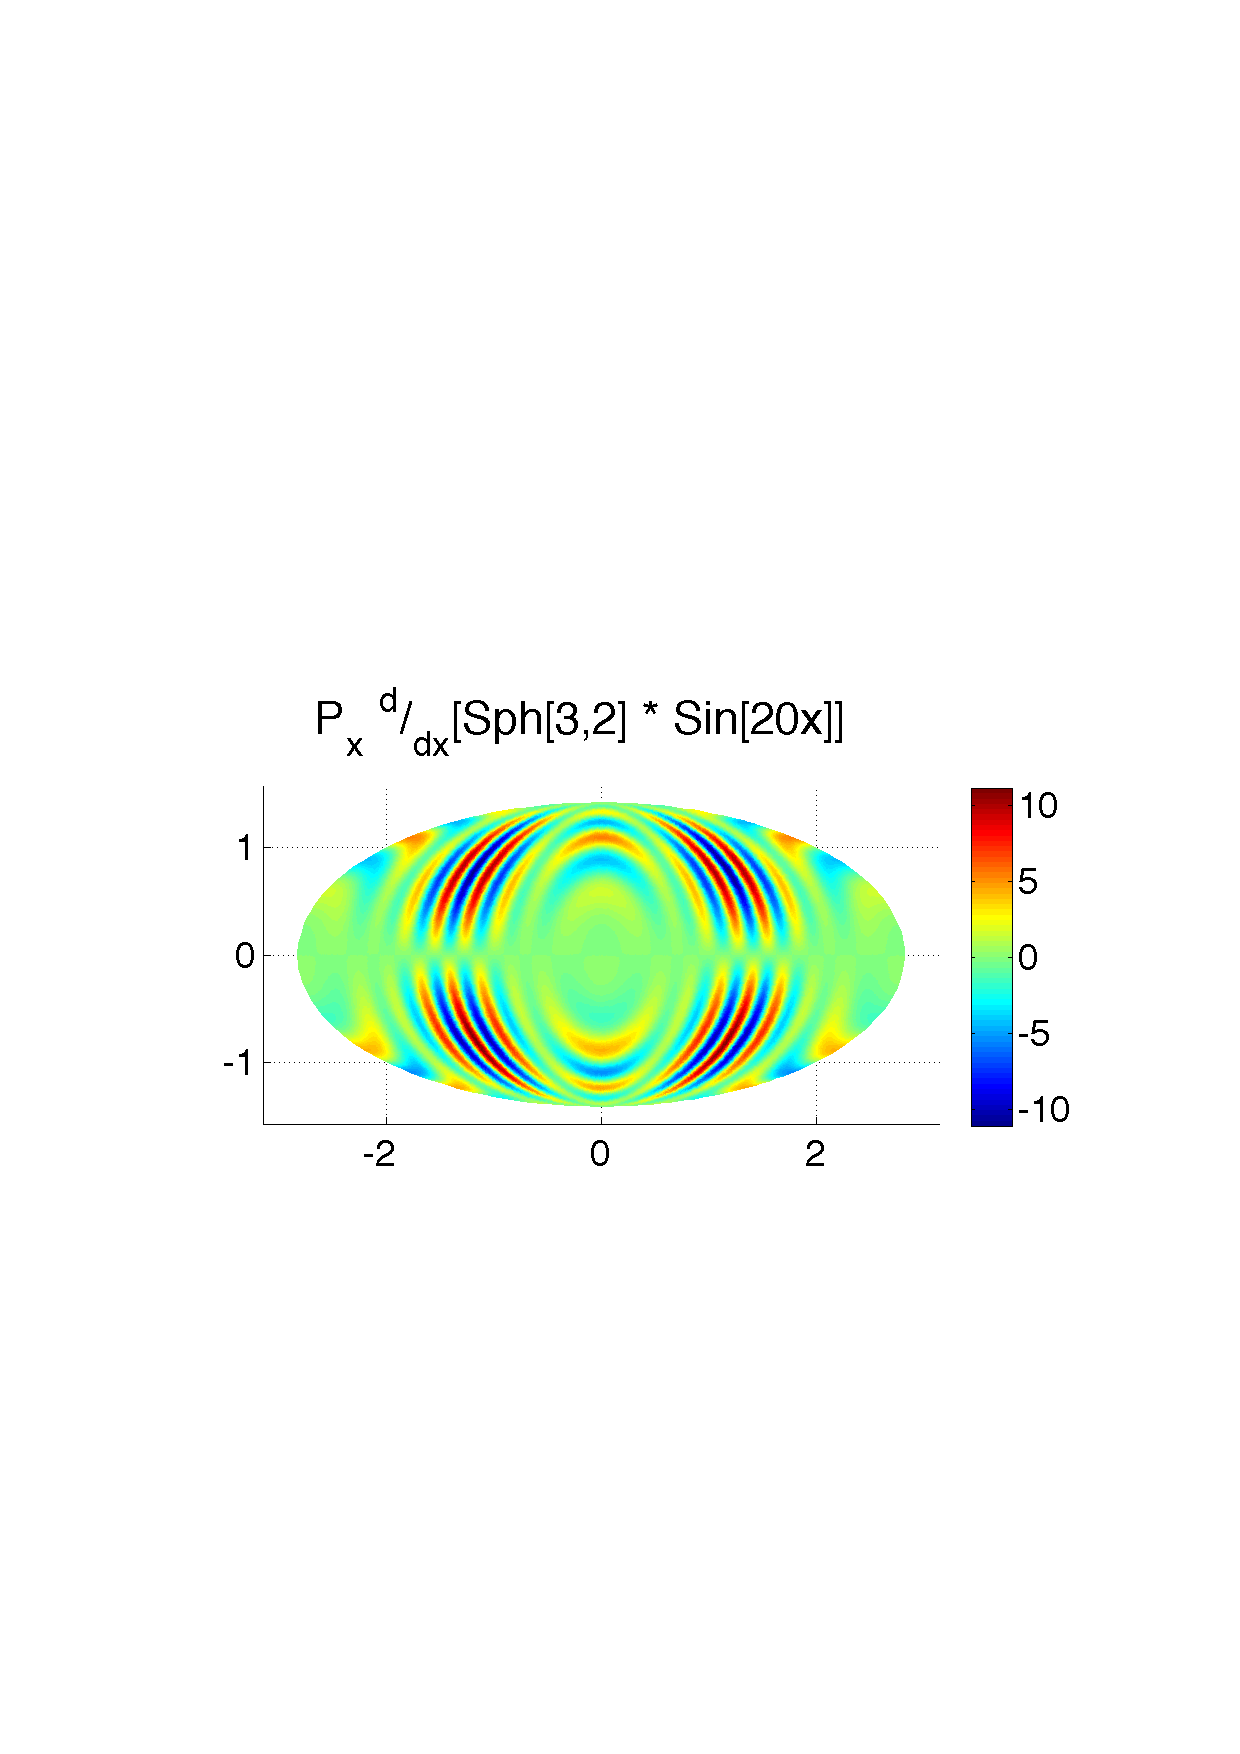
\includegraphics[width=1.0\textwidth]{../figures/chapter2/compare_weight_generation/xsfc_vs_xsfc_alt_on_sph32_times_sine_20x/pdx_sph32_times_sin20x.pdf}
	\caption{$x$-component of the projected gradient: 
	$\mathbf{p}_{x} \cdot \nabla f(\vx)$.  }
	\end{subfigure}
	
	\begin{subfigure}[b]{0.425\textwidth}
	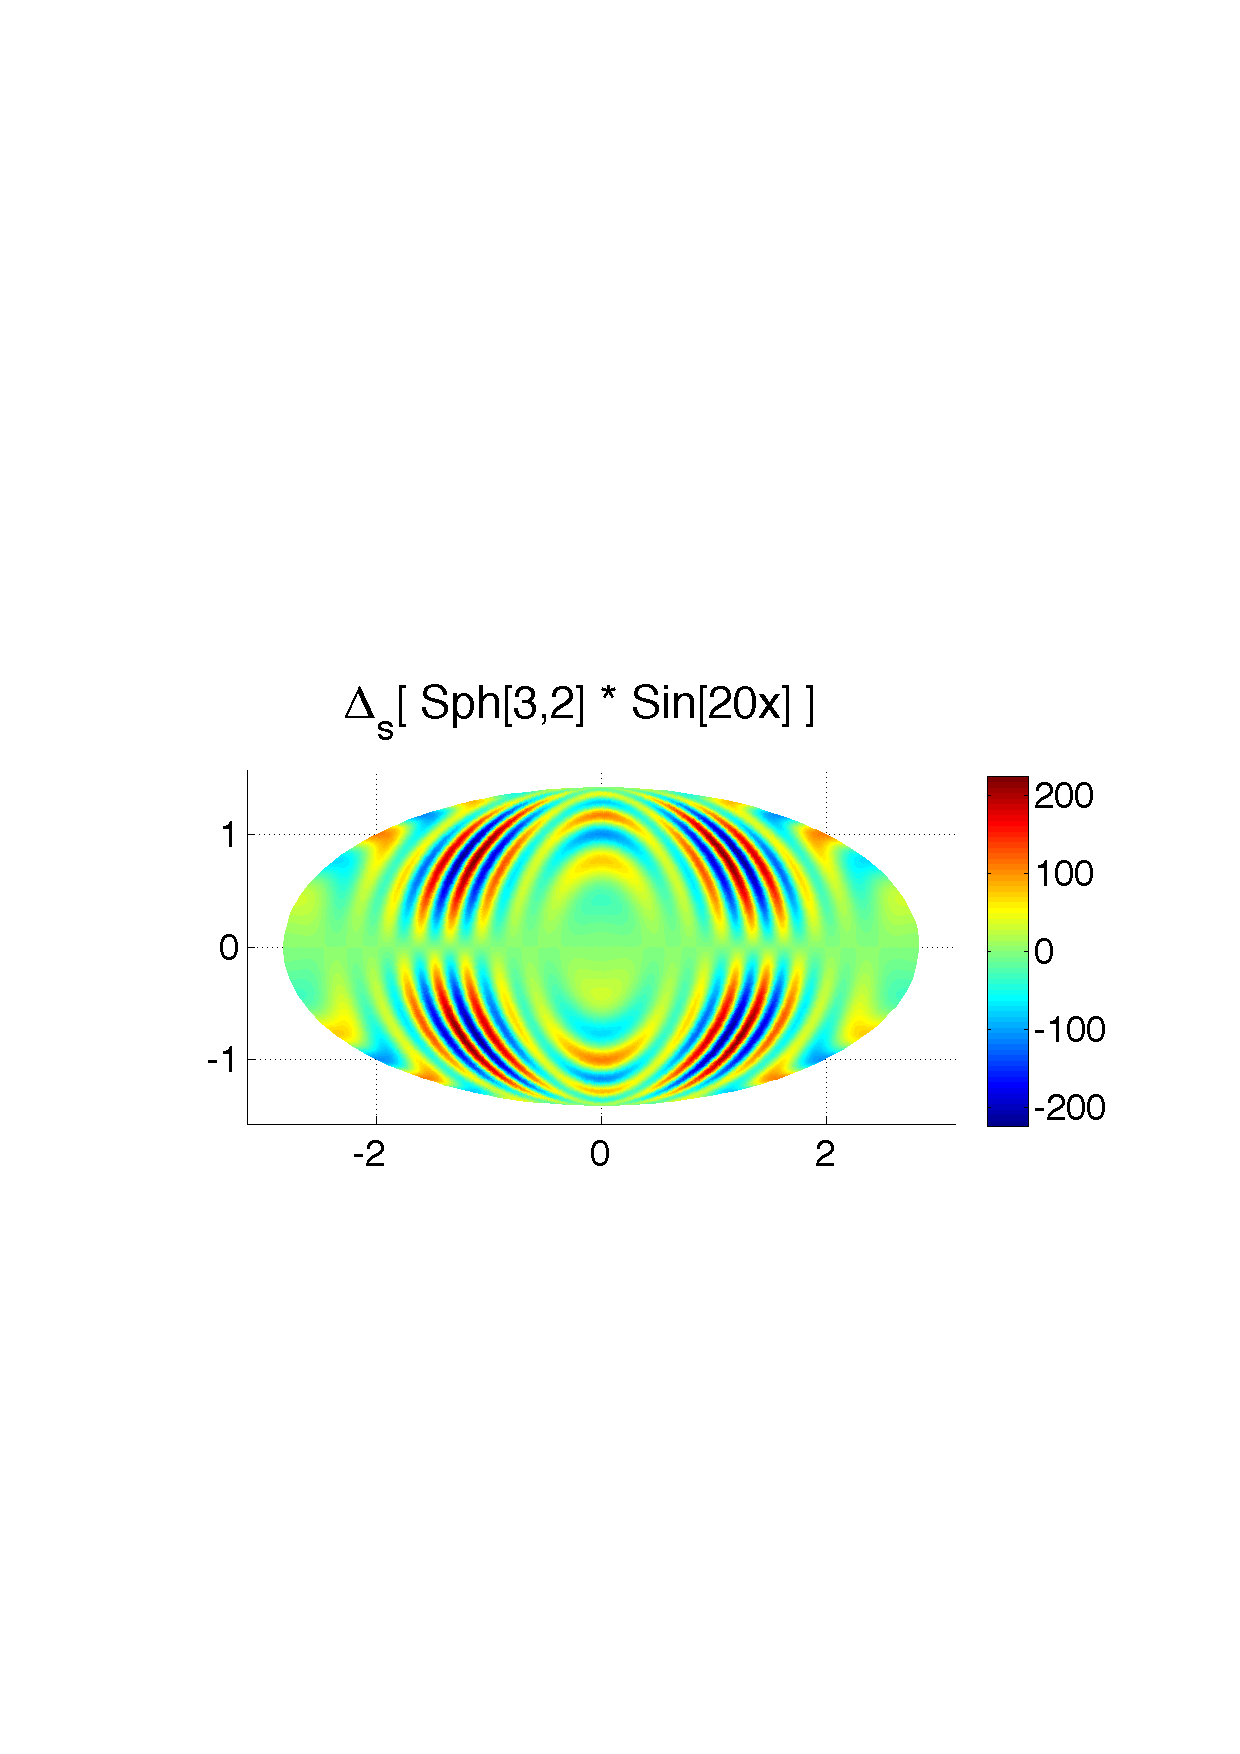
\includegraphics[width=1.0\textwidth]{../figures/chapter2/compare_weight_generation/lsfc_vs_px_grad_dot_px_grad/lsfc_sph32_times_sin20x.pdf}
	\caption{Surface Laplacian: $\LaplaceBeltrami f(\vx)$.  }
	\end{subfigure}
	\caption{Test function and its projected derivatives on the surface of the unit sphere. }
\end{figure}

\begin{figure}[htbp]
	\centering
	\begin{subfigure}[b]{0.425\textwidth}
	\includegraphics[width=1.0\textwidth]{../figures/chapter2/compare_weight_generation/lsfc_vs_px_grad_dot_px_grad/direct_rel_l2_error.pdf}
	\caption{$\LaplaceBeltrami$ of $Y_{3}^{2} \sin(20 x)$}
		\end{subfigure}
	\begin{subfigure}[b]{0.425\textwidth}
	\includegraphics[width=1.0\textwidth]{../figures/chapter2/compare_weight_generation/xsfc_vs_xsfc_alt_on_sph32/direct_rel_l2_error.pdf}
	\caption{$\mathbf{p}_{x} \cdot \nabla ( Y_{3}^{2})$ }
	\end{subfigure}
	\begin{subfigure}[b]{0.425\textwidth}
	\includegraphics[width=1.0\textwidth]{../figures/chapter2/compare_weight_generation/xsfc_vs_xsfc_alt_on_sph32_times_sine_20x/direct_rel_l2_error.pdf}
	\caption{$\mathbf{p}_{x} \cdot \nabla ( Y_{3}^{2} \sin(20 x))$ \authnote{rescale 1e0 down to 1e-8} }
	\end{subfigure}
	\caption{Relative $\ell_{2}$ error in differentiation.}
\end{figure}


\begin{figure}[htbp]
	\centering
	\begin{subfigure}[b]{0.425\textwidth}
	\includegraphics[width=1.0\textwidth]{../figures/chapter2/compare_weight_generation/lsfc_vs_px_grad_dot_px_grad/diff_of_rel_l2_errors.pdf}
	\caption{$\LaplaceBeltrami$ of $Y_{3}^{2} \sin(20 x)$}
	\end{subfigure}
	\begin{subfigure}[b]{0.425\textwidth}
	\includegraphics[width=1.0\textwidth]{../figures/chapter2/compare_weight_generation/xsfc_vs_xsfc_alt_on_sph32/diff_of_rel_l2_errors.pdf}
	\caption{$\mathbf{p}_{x} \cdot \nabla ( Y_{3}^{2})$ }
	\end{subfigure}
	\begin{subfigure}[b]{0.425\textwidth}
	\includegraphics[width=1.0\textwidth]{../figures/chapter2/compare_weight_generation/xsfc_vs_xsfc_alt_on_sph32_times_sine_20x/diff_of_rel_l2_errors.pdf}
	\caption{$\mathbf{p}_{x} \cdot \nabla ( Y_{3}^{2} \sin(20 x))$}
	\end{subfigure}
	\caption{Signed differences of relative $\ell_{2}$ errors in differentiation between Direct and Indirect weights.}
\end{figure}


\begin{figure}[htbp]
	\centering
	\begin{subfigure}[b]{0.425\textwidth}
	\includegraphics[width=1.0\textwidth]{../figures/chapter2/compare_weight_generation/lsfc_vs_px_grad_dot_px_grad/abs_diff_of_rel_l2_errors.pdf}
	\caption{$\LaplaceBeltrami$ of $Y_{3}^{2} \sin(20 x)$}
	\end{subfigure}
	\begin{subfigure}[b]{0.425\textwidth}
	\includegraphics[width=1.0\textwidth]{../figures/chapter2/compare_weight_generation/xsfc_vs_xsfc_alt_on_sph32_times_sine_20x/abs_diff_of_rel_l2_errors.pdf}
	\caption{$\mathbf{p}_{x} \cdot \nabla ( Y_{3}^{2} \sin(20 x))$}
	\end{subfigure}
		\caption{Absolute differences of relative $\ell_{2}$ errors in differentiation between Direct and Indirect weights.}
\end{figure}

%% NOT USEFUL: %%
%\begin{figure}[htbp]
%\centering
%\includegraphics[width=0.425\textwidth]{../figures/chapter2/compare_weight_generation/xsfc_vs_xsfc_alt_on_sph32/condest_dm_xsfc.pdf}
%\caption{Condition number estimates (condest) of direct $\mathbf{p}_{x}\nabla$ differentiation matrix}
%\end{figure}



\section{Test Cases} 

We computed direct and indirect approaches for the MD-node sets with size $N = \{121, 256, 400, 841, 1024, 2500, 4096, 6400, 8100, 10201, 16384, 27556\}$.

We check the relative error of the approximation: 
$$ \text{relative $\ell_{2}$ error} = \frac{|| f_{approx} - f_{exact} ||_{2} }{ || f_{exact} ||_{2} } $$ 

We also look at the difference of relative errors and its absolute value: 
$$
\text{(relative $\ell_{2}$ error)}_{\text{direct}} - \text{(relative $\ell_{2}$ error)}_{\text{indirect}}
$$

We find that our indirect approach functions well compared to the direct method. For small node sizes ($N < 2500$ nodes) we see that the direct method has the advantage with 

\section{Conclusions}

Although it is clear the indirect method functions well compared to the direct method, we must consider its usefulness. Typically, weights are computed only as necessary for the PDE. If the PDE is on the sphere, then directly computing the $\mathbf{P}\cdot \nabla$ operator would be most efficient for both memory and computation. However, one could imagine a scenario such as a 3-D spherical shell domain with physics on the boundaries that must be constrained to the surface, while the interior requires only an unprojected $\nabla$ operator. In such cases, by simply computing for the $\nabla$ operator, we assemble all necessary operators with minimal loss of accuracy and significant savings ($3Nn$ doubles) in storage. 

\authnote{Plot file size of matrix market file to give an idea of how much memory is saved by cutting out operators} 

With $N=1e6$ nodes and stencil size $n=101$, the matrix market file for weights is approximately 1.6 GB on disk. For a GPU with only 6 GB of global memory space available, it is worthwhile to consider possibilities for memory conservation. 


\authnote{Check to see $\nabla \cdot \nabla$ accuracy for heat equation.} 
